\subsection{Testbed and Protocol}
\label{sec:sim}

\begin{table}[t]
\centering
\caption{Ablation over seeds 16--30: five triggers (75 runs) and no trigger (15 runs). Jam-free: runs with no jam. Jam: jammed segment-minutes per run. Throughput (veh/h) and travel time in the network (veh-h): absolute for no control, otherwise the change against it on the same seeds. No gate and true occupancy: the global-local advisory without its gate, and with the camera replaced by the true occupancy in its window.}
\label{tab:main}
\footnotesize
\setlength{\tabcolsep}{2.2pt}
\begin{tabular}{@{}lrrrrr@{}}
\toprule
 & \multicolumn{4}{c}{Five triggers} & No trigger \\
\cmidrule(lr){2-5}\cmidrule(l){6-6}
Controller & Jam-free & Jam & Throughput & Travel time & Throughput \\
\midrule
No control & 1 & 130.8 & 3,456 & 1,622 & 3,546 \\
Feed lookahead & 46 & 11.6 & $-5.4$\% & $+11.9$\% & $-20.8$\% \\
Plan only & 39 & 22.1 & $+2.6$\% & $-10.0$\% & $-2.9$\% \\
Camera only & 5 & 95.5 & $+1.3$\% & $-1.1$\% & $-0.9$\% \\
No gate & 51 & 4.4 & $+2.5$\% & $-6.0$\% & $-6.9$\% \\
\textbf{Global-local} & \textbf{56} & \textbf{3.9} & $\mathbf{+3.9}$\% & $\mathbf{-12.6}$\% & $\mathbf{-3.0}$\% \\
True occupancy & 58 & 3.4 & $+4.3$\% & $-14.3$\% & $-3.0$\% \\
\bottomrule
\end{tabular}
\end{table}

\begin{figure}[t]
\centering
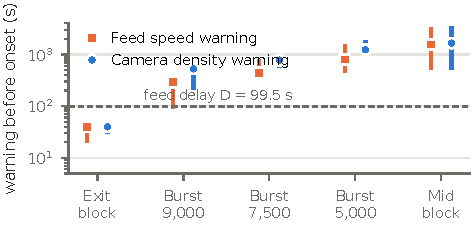
\includegraphics[width=\linewidth]{figs/fig_warning.pdf}
\caption{How early each signal warns. For the first super-segment to jam in each no-control run (14 or 15 runs per trigger), the time before onset at which the feed's speed first fell below 80\% of its pre-trigger level, and at which the camera's density estimate first rose three standard deviations above its own, each held for 30\,s. Markers are medians and bars interquartile ranges; the dashed line is the feed delay $D$.}
\label{fig:warning}
\end{figure}

\begin{figure}[t]
\centering
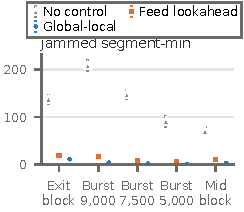
\includegraphics[width=\linewidth]{figs/fig_jams.pdf}
\caption{Jam time by trigger, ordered by how soon no control jams: jammed segment-minutes on the network and its approach roads, mean and two standard errors over 15 seeds.}
\label{fig:jams}
\end{figure}
\begin{figure}[t]
\centering
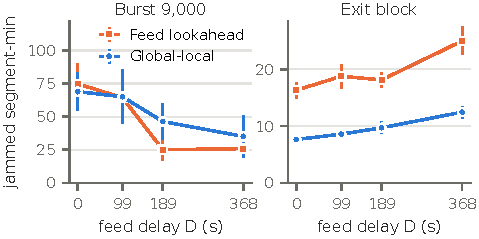
\includegraphics[width=\linewidth]{figs/fig_lag.pdf}
\caption{Jam time against the feed delay $D$, mean and two standard errors over 15 seeds. No control reads no feed and is not shown; it left 213.0 and 137.1 jammed segment-minutes.}
\label{fig:lag}
\end{figure}

\noindent\textbf{Network.} We use the model of the Mainz highway network from~\cite{self_regulating_cars} in SUMO. It has twelve super-segments and ends in an exit where we made three lanes become two, which is where it breaks down. On a real road a vehicle that slows at an entrance also slows the vehicles behind it, so we added a 3\,km approach road, split into three super-segments, before each of the eight entrances. SUMO inserts every vehicle at the far end of its approach road, earlier by that road's free-flow travel time, so that without control the network receives the same demand at the same times. A vehicle on an approach road is shown the plan of the entrance it feeds and uses its camera as on the network, so a queue that a controller builds before an entrance is simulated; the longest, 846\,m, never reached the far end of its road. Controlled vehicles follow the advice through SUMO's speed cap, so car-following still brakes for the vehicle ahead; none of the 1,140 controlled runs had a collision.

\noindent\textbf{Triggers.} Every run starts from a background demand of 3,572\,veh/h, which lies between the flow a jammed exit serves and the flow at which a free one breaks down, so the network does not jam by itself and a jam that forms does not drain (Proposition~\ref{prop:drain}). Fifteen minutes in, one of five triggers is applied. Three are bursts that raise the total inflow to 5,000\,veh/h for ten minutes, or to 7,500 or 9,000\,veh/h for five; they fill the network gradually, and under no control the first jam starts a median of 14 to 28 minutes after the burst begins. Two are stopped vehicles that block a road for five minutes: one lane of the exit road, which jams the exit a median of 80\,s later, and two lanes mid-network, which jams it once the queue reaches the exit, a median of 37 minutes later. Each run lasts two hours, and the feed replays the polled Mainz process with $D=99.5$\,s.

\noindent\textbf{Metrics.} A super-segment is jammed when its mean speed is below 19\,km/h, a threshold fitted to the network's speed distribution by the rule of~\cite{bhardwaj2023understanding}, and a jam starts when that state lasts 120\,s. Jam time is the jammed segment-minutes on the network and the approach roads, because a queue moved upstream delays its vehicles as much as one on the network, and a run is jam-free when it has no jam. Throughput is the flow served at the exit. Travel time is measured as total delay, the vehicle-hours all vehicles spend in the network and on the approach roads beyond their free-flow travel time; the demand is the same for every controller, so a difference in delay is a difference in total travel time.

\noindent\textbf{Baselines and protocol.} We compare the global-local advisory of Section~\ref{sec:controller}, the system below, with two baselines. No control lets every vehicle drive at its own desired speed. The feed lookahead is the controller one would build from the feed alone: it reads the whole network from the same delayed feed and advises 0.5 of the limit when the next super-segment downstream has a jam factor of 2 or more, and 0.75 when the one after it has. All controllers run at full penetration on the same 15 evaluation seeds. Every threshold was chosen on five separate selection seeds, on the network without approach roads, before any evaluation seed ran. We report means over seeds and, for differences, the paired mean with two standard errors.

\subsection{The Camera Warns Before the Feed}
\label{sec:warn}

On the three bursts the camera's density warning came first on 43 of 45 runs, by a median of 200 to 480\,s (Fig.~\ref{fig:warning}). The reason is the shape of the speed-density relation: as occupancy rises to 0.05 the median segment speed falls only from 57.5 to 55.0\,km/h, and then to 35.8\,km/h by 0.07. On the exit block the feed's warning was shorter than $D$ on all 15 runs, so by Proposition~\ref{prop:lag} no controller that reads only the feed could change a speed before that jam began.

\subsection{Jams Prevented and Jam Time}
\label{sec:prevent}

Over the 75 triggered runs no control jammed on 74. The system was jam-free on 41, preventing the jam on 40 runs on which no control jammed, and cut the mean jam time from 131.7 to 16.0 segment-minutes per run, by 88\% (Table~\ref{tab:main}, Fig.~\ref{fig:jams}). It left less jam than no control on all 15 seeds of every trigger, by 68.8 to 148.0 segment-minutes. It prevented every jam after the 5,000\,veh/h burst, 13 of 15 after the 7,500\,veh/h burst and 12 of 14 after the mid-network block, and after the exit block, which jams within 80\,s, it prevented none but shortened the jam from 137.1 to 8.6 segment-minutes.

Against the feed lookahead the system left 29\% less jam over all triggers ($-6.6\pm3.9$ segment-minutes), and less after four of five triggers, by 6.0 to 10.2 (at most $\pm$4.4). After the largest burst the two left the same jam time ($+0.7\pm18.4$), and for both most of it sat on the last kilometre before one of the two entrances nearest the exit (Table~\ref{tab:main}, Upstream). On the network itself the system left 12.6 segment-minutes against no control's 208.4: on that burst both controllers turned a jam on the network into a queue before an entrance rather than removing it.

\subsection{Throughput and Travel Time}
\label{sec:cost}

Over the triggered runs the system served 2.5\% more traffic than no control ($\pm$0.3\%), between 1.0\% and 4.1\% depending on the trigger, at the cost of 1.6\% more total delay ($\pm$1.4\%). The delay depends on how long the prevented jam would have lasted. After the exit block the jam the system shortened cost more than its slowing, and its delay was 2.8\% below no control's ($\pm$1.7\%); after the two larger bursts the difference was within noise; after the 5,000\,veh/h burst and the mid-network block, whose jams under no control are the shortest, the slowing cost more than the jam, 6.5\% and 7.6\% more delay.

The lookahead served 5.4\% less traffic than no control and added 27.9\% to its delay, so the system served 8.3\% more traffic than the lookahead and spent 20.5\% less delay. The difference is what each one slows. The lookahead slows every vehicle upstream of a segment the feed reports as slowing, whether or not that vehicle's own road is filling. The local layer slows only the vehicles whose road ahead is filling, by one step, and changed the advised speed on 17\% of vehicle ticks.

\subsection{Sensitivity}
\label{sec:sens}

\noindent\textbf{Camera distance scale.} We repeated the largest burst and the exit block with every camera distance scaled by 0.8 and by 1.25, since the absolute scale is assumed (Section~\ref{sec:road}). On the exit block it still left 9.3 to 10.4 fewer jammed segment-minutes than the lookahead. On the burst it left 37.0 fewer at 1.25 ($\pm$16.8), but at 0.8, which reads the road as fuller and changed the advised speed on 24\% of vehicle ticks instead of 19\%, it left 60.4 more ($\pm$23.6).

\noindent\textbf{Share of drivers who follow.} With 75\% of vehicles following, the system still left less jam than no control on both triggers. With 50\% it left 27.2 more jammed segment-minutes than no control on the burst ($\pm$24.5), though 34.5 fewer on the exit block ($\pm$19.7).

\noindent\textbf{Feed delay.} We varied the feed delay $D$ (Fig.~\ref{fig:lag}): 0, 99.5, 189 and 368\,s, the last close to the probe latency of~\cite{wang2018latency} plus the measured delivery lag. On the exit block, which jams faster than the feed reports, both controllers left more jam at the longest delay than with none, and the system stayed below the lookahead at every delay. On the largest burst the lookahead's jam time instead fell as $D$ grew, from 74.8 to about 25 segment-minutes at 189 and 368\,s, and at 189\,s it was 21.3 below the system's ($\pm$16.9) while serving 251\,veh/h less; we have not identified why a later feed helps it there.

\subsection{When No Jam Would Have Formed}
\label{sec:notrigger}

The local layer acts on the density ahead without knowing whether a jam would have formed, so it also slows vehicles that did not need slowing. We measured this cost separately, on runs with the background demand and no trigger, where no controller jams. The correction changed the advised speed on 15\% of vehicle ticks, which reduced throughput by 6.9\% (245\,veh/h) and added 29.2\% to the total delay (136 vehicle-hours) relative to no control; the lookahead reduced throughput by 20.8\% and added 42.9\%. Enabling the local layer only when the feed reports the network near capacity is a direct way to reduce this cost, and we leave it to future work.
